\documentclass[tikz,border=8pt]{standalone}
\usepackage[OT4,plmath]{polski}
\usepackage{amsmath}
\begin{document}
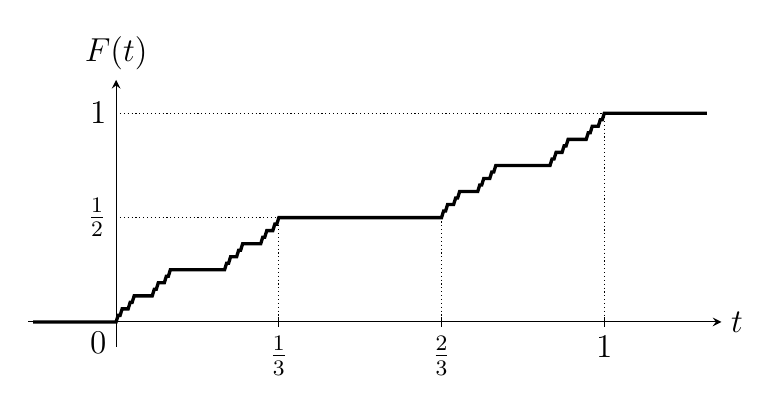
\begin{tikzpicture}[x=6.2cm,y=2.65cm,>=stealth,font=\large]
  \draw[->] (-.18,0)--(1.24,0) node[right] {$t$};
  \draw[->] (0,-.12)--(0,1.16) node[above] {$F(t)$};
  \node[left] at (0,1) {$1$};
  \node[left] at (0,.5) {$\frac12$};
  \node[below left] at (0,0) {$0$};
  \draw ({1/3},.022)--({1/3},-.022) node[below] {$\frac13$};
  \draw ({2/3},.022)--({2/3},-.022) node[below] {$\frac23$};
  \draw (1,.022)--(1,-.022) node[below] {$1$};
  \draw[densely dotted] (0,.5)--({1/3},.5)--({1/3},0)
    ({2/3},.5)--({2/3},0) (0,1)--(1,1)--(1,0);
  % Odcinki liniowe na przedziałach piątego etapu konstrukcji.
  \draw[very thick] plot coordinates {
    (-.17,0)
    ({0/243},{0/32}) ({1/243},{1/32})
    ({2/243},{1/32}) ({3/243},{2/32})
    ({6/243},{2/32}) ({7/243},{3/32})
    ({8/243},{3/32}) ({9/243},{4/32})
    ({18/243},{4/32}) ({19/243},{5/32})
    ({20/243},{5/32}) ({21/243},{6/32})
    ({24/243},{6/32}) ({25/243},{7/32})
    ({26/243},{7/32}) ({27/243},{8/32})
    ({54/243},{8/32}) ({55/243},{9/32})
    ({56/243},{9/32}) ({57/243},{10/32})
    ({60/243},{10/32}) ({61/243},{11/32})
    ({62/243},{11/32}) ({63/243},{12/32})
    ({72/243},{12/32}) ({73/243},{13/32})
    ({74/243},{13/32}) ({75/243},{14/32})
    ({78/243},{14/32}) ({79/243},{15/32})
    ({80/243},{15/32}) ({81/243},{16/32})
    ({162/243},{16/32}) ({163/243},{17/32})
    ({164/243},{17/32}) ({165/243},{18/32})
    ({168/243},{18/32}) ({169/243},{19/32})
    ({170/243},{19/32}) ({171/243},{20/32})
    ({180/243},{20/32}) ({181/243},{21/32})
    ({182/243},{21/32}) ({183/243},{22/32})
    ({186/243},{22/32}) ({187/243},{23/32})
    ({188/243},{23/32}) ({189/243},{24/32})
    ({216/243},{24/32}) ({217/243},{25/32})
    ({218/243},{25/32}) ({219/243},{26/32})
    ({222/243},{26/32}) ({223/243},{27/32})
    ({224/243},{27/32}) ({225/243},{28/32})
    ({234/243},{28/32}) ({235/243},{29/32})
    ({236/243},{29/32}) ({237/243},{30/32})
    ({240/243},{30/32}) ({241/243},{31/32})
    ({242/243},{31/32}) ({243/243},{32/32})
    (1.21,1)
  };
\end{tikzpicture}
\end{document}
